\documentclass{article}
\usepackage[legalpaper, landscape, margin=3cm]{geometry}
\usepackage{xcolor}
\usepackage{amsmath}
\usepackage{amssymb}
\usepackage{tikz}
\usetikzlibrary{arrows,automata,positioning}


\begin{document}
	Formula file: \texttt{Problem10\_label59\_true-unreach-call.c\_69.smt2}

	Two asserts present: $\phi, \psi$

	Assert $\phi$:
	\begin{flalign}
		\phi &: \;\;  \phi_1 \lor \phi_2 \\
		%
		\phi_1 &: \;\;
			3 \le x
			\land
			\exists u, w
				\left(
					23 \le w   							    \color{red} \land \color{black}
					(u \; mod \; 299993) \le v + 300007     \color{red} \land \color{black}
					0 \le u 							    \color{red} \land \color{black}
					5w + 517989 \le u 					
				\right) \\
		%
		\phi_2 &: \;\;
			3 \le x
			\land
			\exists w, y
				\left(
					(y \; mod \; 299993) \le v + 600000 \color{red} \land \color{black}
					23 \le w   							\color{red} \land \color{black}
					(y \; mod \; 299993) \not= 0 		\color{red} \land \color{black}
					y < 0 								\color{red} \land \color{black}
					5w + 517989 \le u 					
				\right)
	\end{flalign}

	Assert $\psi$:
	\begin{flalign}
		\psi &: \;\; \psi_1 \lor \psi_2 \\
		%
		\psi_1 &: \;\;
			3 \le x \land 
			\exists y 
				\left( 
					z \le y 							\color{red} \land \color{black}
					(y\;mod\;299993) \le v + 600000 	\color{red} \land \color{black}
					(y\;mod\;299993) \not= 0 			\color{red} \land \color{black}
					y < 0                               
			\right) \\
		%
		\psi_2 &: \;\;
			3 \le x \land 
			\exists y 
				\left( 
					\underbrace{z \le y 				\color{red} \land \color{black}
								0 \le y 				\color{red} \land \color{black}
								(y\;mod\;299993) \le v + 300007}_{\text{Fragment for the experimentation}}
			\right) 
	\end{flalign}

	\begin{align}
		\alpha &: \;\; z \le y \land 0 \le y \land \underbrace{(y\;mod\;299993) \le v + 300007}_{\color{red}\text{Existential quantif.}} \\
			   &\leadsto \color{red} \exists m \color{black} 
			   \left( 
					\underbrace{z \le y \land
								0 \le y \land 
								\color{red}m\color{black} \le v + 300007}_{\text{Linear}} \color{red}\land 
					\underbrace{y \equiv_{299993} m}_{\color{black}\text{Counter}} \color{black}\right)
	\end{align}

\tikzset {
	->,
	>=stealth',
	initial text=$ $,
}

\begin{figure}[ht]
	\center
	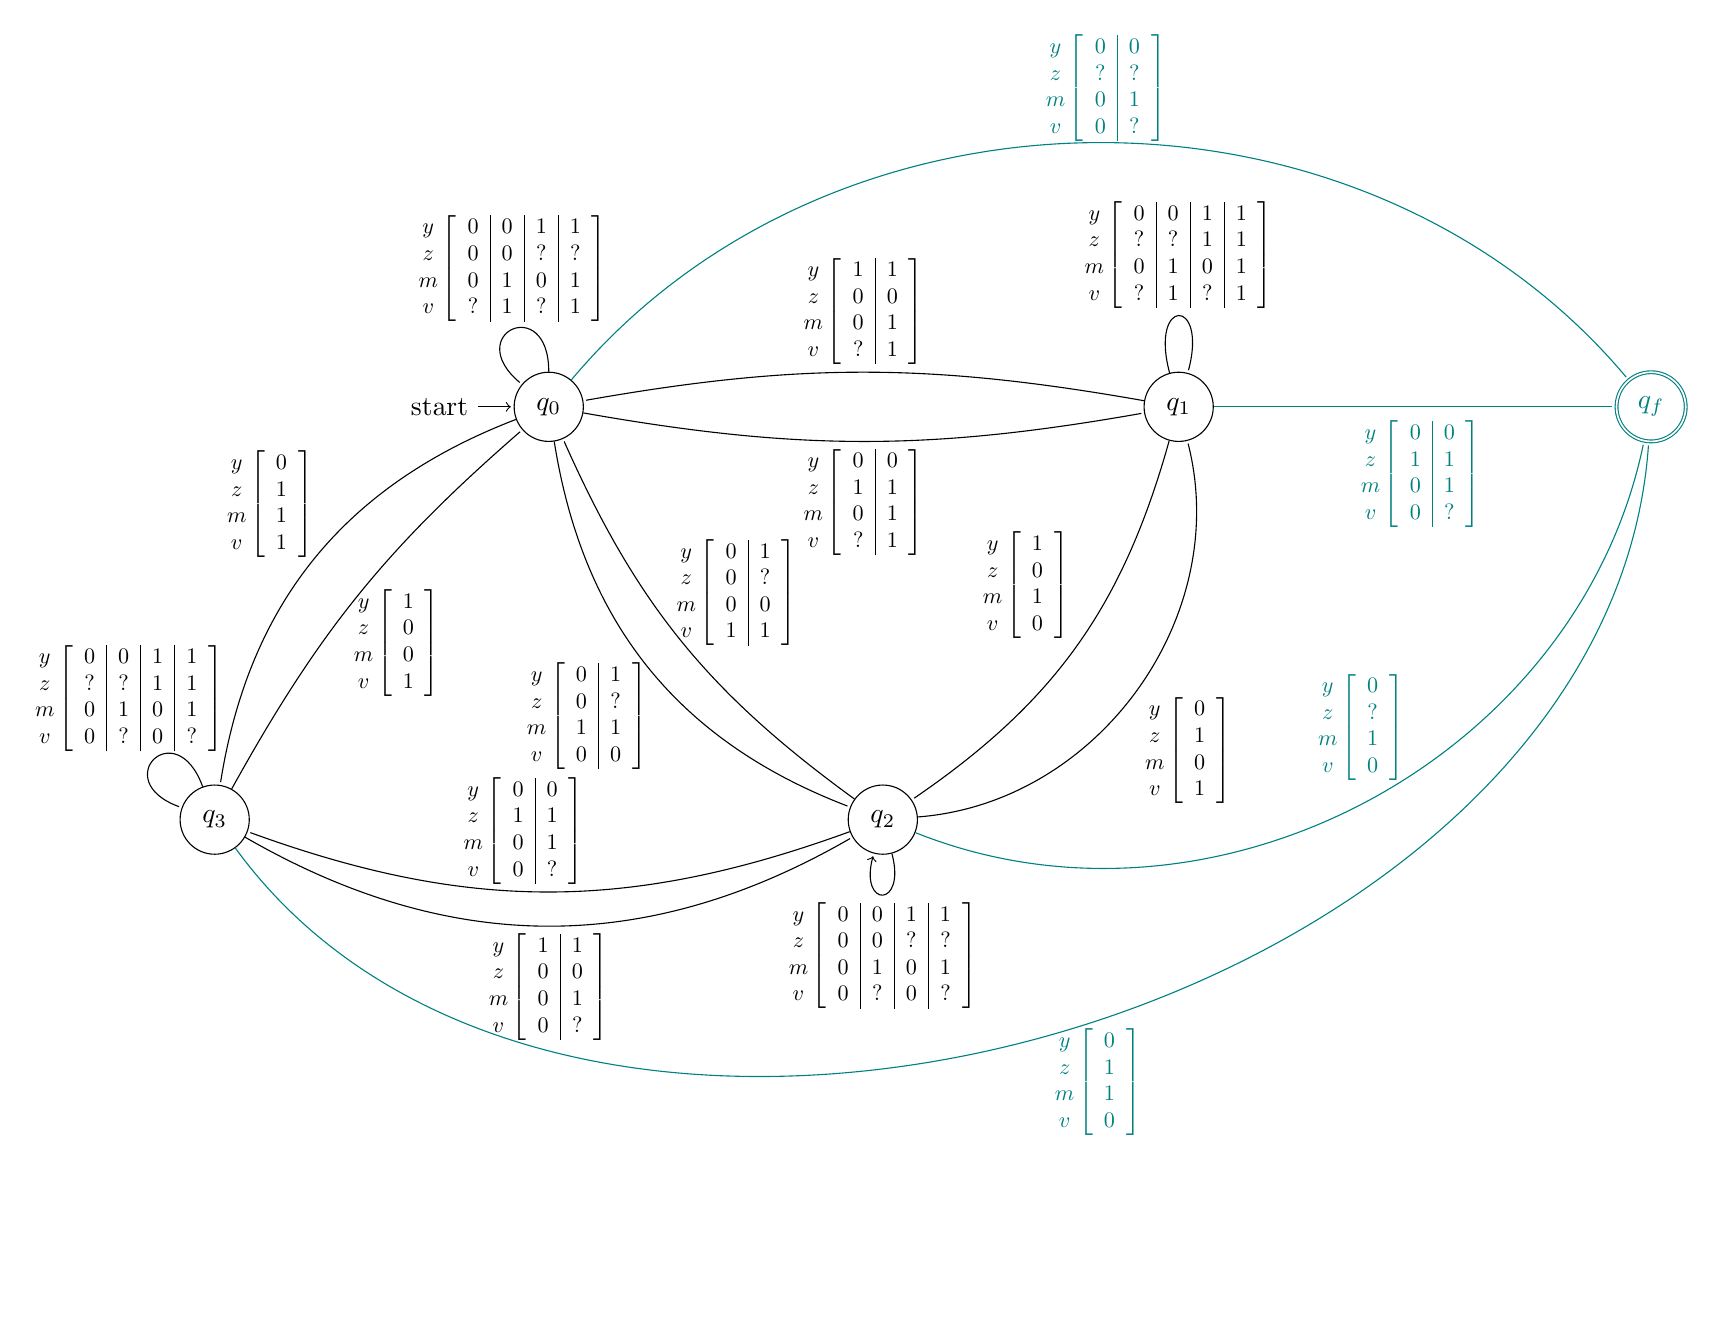
\begin{tikzpicture}[shorten >=1pt, node distance = 6cm]
		\node[state, initial] (q_0) {$q_0$};
		\node[state, right of=q_0] at ++(2cm, 0) (q_1) {$q_{1}$}; 
		\node[state, below right of=q_0] at ++(0, -1cm) (q_2) {$q_2$}; 
		\node[state, below left of=q_0] at ++(0, -1cm) (q_3) {$q_3$}; 
		\node[state, right of=q_1, accepting, teal] (q_f) {$q_f$}; 

		\begin{scope}[every node/.style={scale=0.8}]
			\draw 	(q_0) 
					edge[loop above, distance=1cm, out=90, in=140] 
					node {$
						\begin{matrix}
							y \\
							z \\
							m \\
							v
						\end{matrix}
						\left[
							\begin{array}{c|c|c|c}
								0 & 0 & 1 & 1 \\
								0 & 0 & ? & ? \\
								0 & 1 & 0 & 1 \\
								? & 1 & ? & 1
							\end{array}
						\right]
					$}
				(q_0)
				(q_0)
					edge[bend right=10, below] 
					node {$
						\begin{matrix}
							y \\
							z \\
							m \\
							v
						\end{matrix}
						\left[
							\begin{array}{c|c}
								0 & 0 \\
								1 & 1 \\
								0 & 1 \\
								? & 1
							\end{array}
						\right]
					$}
				(q_1)
				(q_1)
					edge[loop above, distance=1cm] 
					node {$
						\begin{matrix}
							y \\
							z \\
							m \\
							v
						\end{matrix}
						\left[
							\begin{array}{c|c|c|c}
								0 & 0 & 1 & 1\\
								? & ? & 1 & 1\\
								0 & 1 & 0 & 1\\
								? & 1 & ? & 1
							\end{array}
						\right]
					$}
				(q_1)
				(q_1)
					edge[bend right=10, above] 
					node {$
						\begin{matrix}
							y \\
							z \\
							m \\
							v
						\end{matrix}
						\left[
							\begin{array}{c|c}
								1 & 1 \\
								0 & 0 \\
								0 & 1 \\
								? & 1
							\end{array}
						\right]
					$}
				(q_0)
				(q_0)
					edge[bend right=30, below left] 
					node [xshift=0.1cm,yshift=0.2cm]{$
						\begin{matrix}
							y \\
							z \\
							m \\
							v
						\end{matrix}
						\left[
							\begin{array}{c|c}
								0 & 1 \\
								0 & ? \\
								1 & 1 \\
								0 & 0
							\end{array}
						\right]
					$}
				(q_2)
				(q_2)
					edge[bend left=15, above right] 
					node [xshift=-0.2cm,yshift=-0.2cm]{$
						\begin{matrix}
							y \\
							z \\
							m \\
							v
						\end{matrix}
						\left[
							\begin{array}{c|c}
								0 & 1 \\
								0 & ? \\
								0 & 0 \\
								1 & 1
							\end{array}
						\right]
					$}
				(q_0)
				(q_1)
					edge[bend left=20, above left] 
					node[] {$
						\begin{matrix}
							y \\
							z \\
							m \\
							v
						\end{matrix}
						\left[
							\begin{array}{c}
								1  \\
								0  \\
								1  \\
								0 
							\end{array}
						\right]
					$}
				(q_2)
				(q_2)
					edge[bend right=50, below right] 
					node[] {$
						\begin{matrix}
							y \\
							z \\
							m \\
							v
						\end{matrix}
						\left[
							\begin{array}{c}
								0  \\
								1  \\
								0  \\
								1 
							\end{array}
						\right]
					$}
				(q_1)
				(q_2)
					edge[loop below] 
					node[] {$
						\begin{matrix}
							y \\
							z \\
							m \\
							v
						\end{matrix}
						\left[
							\begin{array}{c|c|c|c}
								0 & 0 & 1 & 1 \\
								0 & 0 & ? & ? \\
								0 & 1 & 0 & 1 \\
								0 & ? & 0 & ?
							\end{array}
						\right]
					$}
				(q_2)
				(q_3)
					edge[bend right=30, below] 
					node[] {$
						\begin{matrix}
							y \\
							z \\
							m \\
							v
						\end{matrix}
						\left[
							\begin{array}{c|c}
								1 & 1 \\
								0 & 0 \\
								0 & 1 \\
								0 & ?
							\end{array}
						\right]
					$}
				(q_2)
				(q_2)
					edge[bend left=20, above] 
					node[xshift=-0.4cm] {$
						\begin{matrix}
							y \\
							z \\
							m \\
							v
						\end{matrix}
						\left[
							\begin{array}{c|c}
								0 & 0 \\
								1 & 1 \\
								0 & 1 \\
								0 & ?
							\end{array}
						\right]
					$}
				(q_3)
				(q_3)
					edge[loop above, distance=1cm, out=110, in=160] 
					node[xshift=-.4cm] {$
						\begin{matrix}
							y \\
							z \\
							m \\
							v
						\end{matrix}
						\left[
							\begin{array}{c|c|c|c}
								0 & 0 & 1 & 1 \\
								? & ? & 1 & 1 \\
								0 & 1 & 0 & 1 \\
								0 & ? & 0 & ?
							\end{array}
						\right]
					$}
				(q_3)
				(q_3)
					edge[bend left=10, below right] 
					node[xshift=-0.2cm,yshift=0.2cm] {$
						\begin{matrix}
							y \\
							z \\
							m \\
							v
						\end{matrix}
						\left[
							\begin{array}{c}
								1 \\
								0 \\
								0 \\
								1
							\end{array}
						\right]
					$}
				(q_0)
				(q_0)
					edge[bend right=30, above left] 
					node[xshift=0.1cm,yshift=-0.1cm] {$
						\begin{matrix}
							y \\
							z \\
							m \\
							v
						\end{matrix}
						\left[
							\begin{array}{c}
								0 \\
								1 \\
								1 \\
								1
							\end{array}
						\right]
					$}
				(q_3);
			\draw[teal]
				(q_1)
					edge[below] 
					node[xshift=0.1cm,yshift=-0.1cm] {$
						\begin{matrix}
							y \\
							z \\
							m \\
							v
						\end{matrix}
						\left[
							\begin{array}{c|c}
								0 & 0 \\
								1 & 1 \\
								0 & 1 \\
								0 & ?
							\end{array}
						\right]
					$}
				(q_f)
				(q_0)
					edge[bend left=50, above] 
					node[xshift=0.1cm,yshift=-0.1cm] {$
						\begin{matrix}
							y \\
							z \\
							m \\
							v
						\end{matrix}
						\left[
							\begin{array}{c|c}
								0 & 0 \\
								? & ? \\
								0 & 1 \\
								0 & ?
							\end{array}
						\right]
					$}
				(q_f)
				(q_2)
					edge[bend right=50, above] 
					node[xshift=-0.1cm,yshift=0.2cm] {$
						\begin{matrix}
							y \\
							z \\
							m \\
							v
						\end{matrix}
						\left[
							\begin{array}{c}
								0 \\
								? \\
								1 \\
								0
							\end{array}
						\right]
					$}
				(q_f)
				(q_3)
					edge[bend right=70, below right] 
					node[xshift=-0.1cm,yshift=0.2cm] {$
						\begin{matrix}
							y \\
							z \\
							m \\
							v
						\end{matrix}
						\left[
							\begin{array}{c}
								0 \\
								1 \\
								1 \\
								0
							\end{array}
						\right]
					$}
				(q_f)
				;
		\end{scope}
	\end{tikzpicture}
	\vspace{-2cm}
	\caption{SCC of $A_{linear}$}
	\label{fig:automaton_padding_closure}
\end{figure} 
\end{document}
